
%%%%%%%%%%%%%%%%%%%%%%%%%%%%%%%%%%%%%%%%%%%%%%%%%%%%%%%%%%%%%%%%%%%%%%%%%%%%%%%%%%%%%%%%%%%%%%%%%%%%%%%%%%%%%%%%%%%%%
%%%%%%%%%%%%%%%%%%%%%%%%%%%%%%%%%%%%%%%%%%%%%%%%%%%%%%%%%%%%%%%%%%%%%%%%%%%%%%%%%%%%%%%%%%%%%%%%%%%%%%%%%%%%%%%%%%%%%
%%%%%%%%%%%%%%%%%%%%%%%%%%%%%%%%%%%%%%%%%%%%%%%%%%%%%%%%%%%%%%%%%%%%%%%%%%%%%%%%%%%%%%%%%%%%%%%%%%%%%%%%%%%%%%%%%%%%%

\fancychapter{SIMD Inter-task parallel Viterbi}

\section{Proposed Solution}

The focus of the present work is to develop a parallelization approach based on SIMD (namely SSE on Intel Processors) inter-task vectorization for Profile \acp{HMM} algorithms. Rognes in 2011 (\cite{rognes2011}) pursued this strategy for alignment algorithms like Smith-Waterman. Building on Rognes' work, the same strategy can be followed for \acp{HMM} algorithms. 
However, as mentioned in the previous chapter, this is a promising new approach, that has not yet been much explored.
%this is still a rarely explored avenue which this work hopes to bring into more study. 

This work focuses on one of the most popular \acp{HMM} Homology search suites: HMMER \cite{hmmer3}. HMMER offers many tools, and one of the its key processing steps used by many of the tools is the Viterbi Decoding algorithm with a Profile \ac{HMM}. The Viterbi step is currently (as of May 2013) being implemented on SSE with Farrar's intra-task striped pattern. In this work, an alternative solution was developed, 
%Here, a new alternative solution was developed, that hopes to be competitive against, and improve on, HMMER's existing implementation. 

The Rognes-based implementation of Viterbi Decoding created in this work was named \emph{COPS} (Cache-Oblivious Parallel SIMD Viterbi). It is targeted at the HMMER suite and it is compatible with its internal configurations, being mostly interchangeable with the exception of the requirements of Inter-task parallelism (i.e. processing batches of sequences each time instead of just one). Also for this reason, COPS was developed on top of the HMMER suite as a standalone tool instead of being integrated into the HMMER pipeline of search filters (one of which being the Viterbi algorithm). A full integration into the HMMER pipeline was deemed unsuitable, since the pipeline is designed to process only one sequence at a time. Later work may extend this approach to the Forward algorithm as well and as into AVX2, Intel's new vector instruction set (an  extension of SSE).


%REVER ISTO
The following sections will present the developed implementation of the Viterbi algorithm with inter-task vectorization, the problems found, and two new methods to improve the strategy used by Rognes. Finally, the last section will describe a coarser-grained multi-threading parallelization of the algorithm itself, running on top the vector inter-task parallelization.





%%%%%%%%%%%%%%%%%%%%%%%%%%%%%%%%%%%%%%%%%%%%%%%%%%%%%%%%%%%%%%%%%%%%%%%%%%%%%%%%%%%%%%%%%%%%%%%%%%%%%%%%%%%%%%%%%%%%%
%%%%%%%%%%%%%%%%%%%%%%%%%%%%%%%%%%%%%%%%%%%%%%%%%%%%%%%%%%%%%%%%%%%%%%%%%%%%%%%%%%%%%%%%%%%%%%%%%%%%%%%%%%%%%%%%%%%%%


\section{Rognes-based SSE Inter-task vectorization}
\label{Rognes-based SSE Inter-task vectorization}

The main goal of this work consisted in implementing an inter-task vector parallelization of Viterbi Decoding in Intel's SSE, such as Rognes did for the Smith-Waterman algorithm \cite{rognes2011}.

Recall that this approach consists of using the N parallel SIMD channels for N different references (i.e. computing the Viterbi equations in parallel for the N sequences). This is known as 'Inter-task parallelism', as described previously in \sref{Inter-task Parallelism}. 

The initial implementation was largely based on Rognes' vectorization of the Smith-Waterman algorithm, with the changes necessary for the Viterbi problem. Since it is a form of inter-task parallelism, each channel is expected to perform the same operations, and thus the core of the algorithm maintains mostly the logic of the scalar version. The corresponding code  for the inner loop over the model states is presented in \cref{code-rognes}.

	
Initially, 32-bit floating-point values were used, which allowed for four independent channels in the SSE vectors. Four different sequences are fed into these four channels. Mmx, Imx and Dmx are the SSE dynamic programming arrays, respectively for Match, Delete and Insert state values. Mpv, Ipv and Dpv are auxiliary SSE registers to temporarily hold delayed or preempted values.
vB and vE are the SSE registers for the E and B flanking states values.

To compute the Match states, there are dependencies on M, D, and I, namely from the previous state triplet and previous sequence symbol (Mpv, Dpv, Ipv). These dependencies must be retrieved in the previous state iteration, \emph{before the writes}, to fetch the values of the previous symbol (indexes (i-1, k-1) in a \ac{DP} matrix) before they are re-written.
Each computed Match value is used to update the E (semi-end) state. 

In regards to Insert states, they depend on the M and I values in the same state-triplet, but from the previous sequence token. The M and I values can thus be fetched from the current state iteration, before the updates (saved in Mpv and Ipv).
Note that the D $\rightarrow$ I transitions have been removed by design from the model.

Finally, for the Delete states, there are D $\rightarrow$  D and M $\rightarrow$  D dependencies, from the same sequence token but previous state triplet (indexes (i,k-1)). To find these, it is necessary to preemptively compute and save the D and M values in the previous state iteration (Mnext saved and Dcv preemptively computed).

After each inner loop over the state triplets, the special states (E, J, C, N and B) are updated.


The measured performance (number of values computed per second) is mostly dependent on the model length (denoted by M, number of model state-triplets), with hardly any influence from the sequences length (denoted by L).
It achieved a 78\% performance improvement on the serial version by this initial parallelization with the Rognes-bases strategy. A diagram of the Rognes algorithm applied to HMMER is shown in \autoref{rognes-hmmer}.

\begin{figure}[htb!]
  \begin{center}
    \resizebox*{1.0\columnwidth}{!}{ 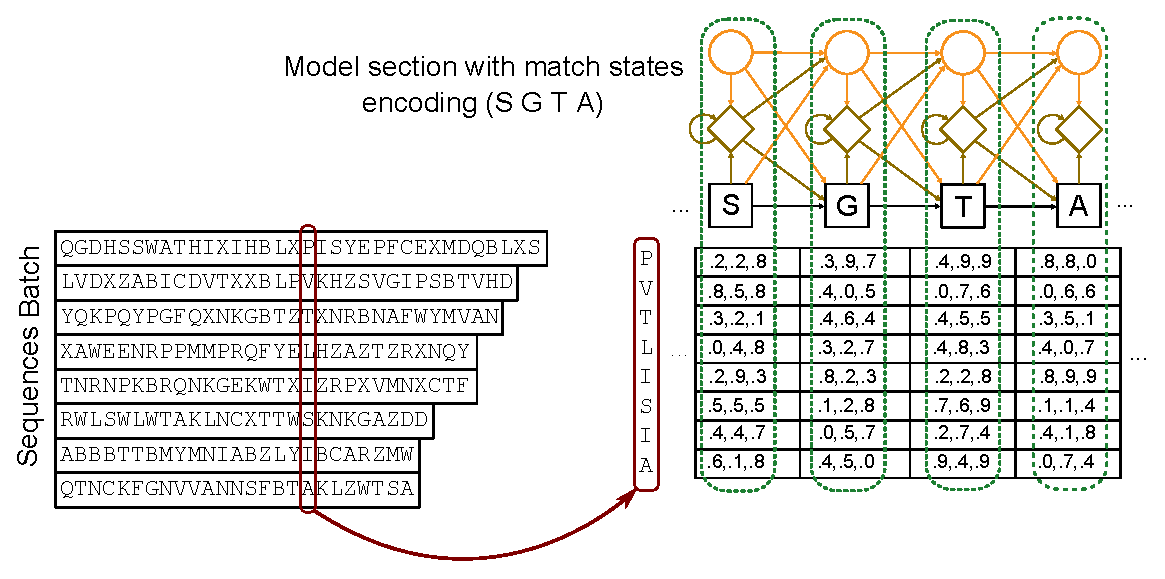
\includegraphics{img/rognes-hmmer.eps} }
    \caption[Vectorization of the Viterbi algorithm] {Rognes inter-sequence strategy applied to Viterbi Decoding in HMMER.}
    \label{rognes-hmmer}
  \end{center}
\end{figure}



\paragraph*{Initial Optimizations to the Rognes strategy}

\begin{itemize}

%The J transitions were removed from the model since our implementation does not support multihit alignments.
%Since our implementation only supports multihit local mode, the J state is disabled. As a result the E $\rightarrow$ C transition is always taken, hence the transition cost is 0 and can be removed from the algorithm.

\item Since the Insert emission scores are set to the background distribution in HMMER by default, they yield a null contribution and can be removed from the code.

\item It is possible is to pre-compute and save the $vB$ values for each state triplet. This however cannot be done when dealing with a dataset composed of varying-length sequences, since the model must be re-configured with each different sequence length.

\item For the main transition scores (i.e. between normal states), a single array was allocated, and the 8 transitions were stored in a interleaved manner, continuous in relation to the state triplets, in the order by which they are fetched in the inner loop. This allows for a better use of memory, avoiding mixed accesses to multiple different memory locations.
This arranged pre-allocated layout yielded a performance speedup of 15\%. 

\item Another improvement is unrolling the last iteration of the inner loop. The last iteration is particular since it only needs to compute the match value, hence the other operations can be removed.

\end{itemize}




\section {Loading of Emission Scores}
\label {Loading of Emission Scores}

Special concern was given to the method of loading and arranging the per-token Match Emission scores, because it was found that this step accounted for a substantial fraction of the overall time spent by the application. First the original method used by Rognes in the Swipe tool was implemented, evaluated, and then a new improved strategy was devised and implemented. The two are analyzed in the following sections.


\subsection{Rognes method of Loading the Emission Scores}

The Match Emission scores present a significant problem: it is impossible to arrange the emission scores in an memory-efficient pattern before the sequence tokens are known. A complete pre-arrangement of all possible $token \times state$ combinations would require $AlphabetSize^{AlphabetSize} \times L \times M$ 16-byte values. For DNA, which has an $AlphabetSize$ of 4, the required memory is manageable. For proteins, which are the usual target of such systems and have an usual $AlphabetSize$ of 21, it exceed the available memory of almost every system.The complete pre-calculation approach is infeasible.

To tackle this problem, initially, the loading of the Match emission scores was done using the method of Rognes' Swipe program \cite{rognes2011}. The method consists in pre-loading and arranging each quartet of emission scores ($4xM$, $M$ being the Model length), corresponding to the 4 parallel sequence tokens, necessary for the entire inner loop through the model states. For each new tuple of sequence tokens, an array of $M$ SSE vectors is computed and arranged for efficient access in the inner loop.

The costly arrangement must compute a transposition of the original scores, in successive rounds of 4x4 32-bit values: arrays indexed by symbol are transposed into consecutive tuples of 4 interleaved scores from the 4 different sequences. The transposition is achieved through SSE \emph{unpack} instructions, which interleave the lower or higher-order bits of 2 arguments, starting with a finer-grain unpack (32-bit unpacks when using 32-bit scores) and proceeding to coarser-grained unpacks (ultimately 64-bit unpacks that compute 128-bit values, size of the SSE vectors). This strategy is illustrated in \autoref{scores-loading-rognes}, with the corresponding pseudo-code shown in \cref{code-loading-rognes}.


\begin{figure}[htb!]
  \begin{center}
    \resizebox*{1.0\columnwidth}{!}{ 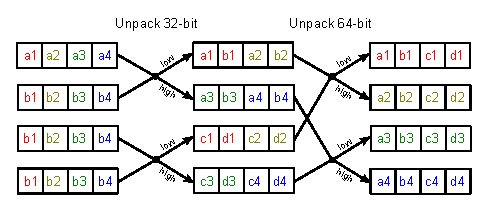
\includegraphics{img/scores-loading-rognes.eps} }
    \caption[Loading of Emission scores] {Emission scores pre-processing using SSE unpacks, according to Rognes' Swipe tool.}
    \label{scores-loading-rognes}
  \end{center}
\end{figure}


%\begin{algorithm}[htb!]
%\caption{ - Exemplo Listing }
%\label{code-listing-rognes}
%
%\lstset{language=C} 
%\begin{lstlisting}
%
%	/* Initialization of the zero row.	*/
%	xmxN = 0;
%	xmxE = xmxJ = xmxC = -eslINFINITY;			/* need seq to get here */
%	for (k = 0; k <= gm->M; k++)
%		dmx[k] = mmx[k] = imx[k] = -eslINFINITY;	/* need seq to get here */
%	/* DP recursion */
%	for (i = 1; i <= L; i++) 
%	{
%		float *rsc = gm->rsc[dsq[i]];
%		float sc, ipv, mpv, dpv, dcv;
%		dcv = mpv = dpv = ipv = sc = -eslINFINITY;
%		imx[0] = dmx[0] = mmx[0] = -eslINFINITY;
%		xmxE = -eslINFINITY;
%	}
%\end{lstlisting}
%\end{algorithm}

Besides the costly SSE operations in themselves, this method suffers from a poor memory utilization, requiring an additional write (and later read) to store and load the re-arranged scores. The results obtained point to roughly 30\% of the program runtime being spent in the arrangement of emission scores, a considerable amount.



\subsection{Inline method of Loading the Emission scores}

The original strategy for the pre-processing of emission scores, as developed by Rognes in Swipe, suffered from a serious performance penalty. In order to relieve this burden,  a new method was devised to keep Emission values as closer to the processor as possible, and thus avoid the drawback of the additional re-writing on memory. 

The transposition of scores is processed by rounds of 4 (since each SSE vector holds 4 floats, and the transposition must use a square 'matrix'), so the round of 4 values is the smallest block of data that can be transposed at the same time. The new method computes these 4-floats transpositions inlined between each round of 4 inner loop iterations. Each transposition produces 4 SSE vectors of emission scores, which can then immediately be used to compute 4 state triplets. The transposed scores are merely stored temporarily in close cache memory, and thus avoid the penalty hit of a full round of memory re-writings and improves the cache efficiency. This requires the inner loop be unrolled in 4 iterations.

After this transformation, the new inner loop consists of the code in \cref{code-loading-inline}. The optimization of interleaved scores' loading lead to an execution time roughly 30\% to 40\% faster than the pre-loading method used by Rognes' tool.

This method requires the number of model states to be a multiple of 4 (for 32-bit floats), to support the 4-state loop step. In order to easily deal with this, the model should be padded with dummy states up to a 4-state barrier. The dummy states carry dummy scores, set to $-infinity$, so that they have a null effect on the final results. These extra dummy states have a negligible effect on the overall performance.





\section{Discretization to 8x16-bit integer channels}

In order to increase the parallelization potential, the original 4 channel x 32-bit float version was converted to an 8channel x 16-bit integer version. This conversion implied a discretization of the floating-point scores, similar to the one employed by HMMER in its Viterbi Filter algorithm.

The discretization used a scale transformation with a factor configurable at compile-time. HMMER's authors estimate an optimal scaling factor of $\frac{500.0}{\ln 2}$, which does not underflow for any $L,M <= 10^{16}$ (\cite{hmmer3}).

Although 16-bit scores do not underflow (for any practical application), they may easily overflow when the sequence is slightly similar to the underlying family of the model. The occurrence of such overflows is detected by numerical manipulation of the vE values at the end of the inner loop.
%\begin{algorithmic}
%\LeftComment Select the overflowed channels
%\State newOverflows = \_mm\_cmpgt\_epi16(xmxE, vLimit)
%\LeftComment Union of the new overflowed channels with the older ones
%\State vOverflows = \_mm\_or\_si128(vOverflows, newOverflows)
%\end{algorithmic}


\myparagraph{3/2-nat optimization}
\label {3/2-nat optimization}

The 3/2-nat optimization was adopted to simplify the special-state calculations, and it is only valid for local alignment:
HMMMER assumes that, for local alignment with reasonable large and non-homologous sequences, only a small section will be matched. The rest of alignment will be merely filled with gaps (NN, CC, and JJ loops), totaling close to $L$ gaps. So, the optimization removes the NN, CC, and JJ loop transitions from the algorithm, and adds the correspondent cumulative sum of their contributions (3.0 for multihit mode and 2.0 for unihit) in the end. 

In COPS, it was equally applied the '-2.0 nat approximation' used by HMMER: N $\rightarrow$ N and C $\rightarrow$ C transitions are deleted, and a -2.0 offset bias is added to N in the beginning, and subtracted after the algorithm finishes. This value approximates the cumulative contribution of N $\rightarrow$ N and C $\rightarrow$ C insertion loops which, for a large $L$, is given by $ \log  \frac{L}{L+2}$.

%Eles substitutim estas transicoes por uma aprox para sequencias longas. No entanto o erro aumenta quando as sequencias sao semelhantes. 



\section{Model Partitioning to improve the L1 cache utilization}
\label{Model Partitioning to improve the L1 cache utilization}

A significant bottleneck was detected in the utilization of the innermost L1 data cache when using large models. This section will analyze the problem, and the solution that was found based on loop-tiling the inner loop.


\subsection{Problems with First-level Cache Efficiency}
\label{Problems with First-level Cache Efficiency}

At this point, early results showed a considerable performance degradation with an increasing Model length. After some experiments, it was found that the deterioration was caused by an exponential increase in the number of occurring L1 cache misses (the fastest cache level in Intel processors). It was also found that these L1D cache misses were overwhelmingly in the core inner loop of the code ($\sim$97\% of total cache misses).

An explanation for the explosion of cache misses seemed likely to be the eviction of the $M$-length auxiliary and scores' arrays from the cache between each execution of the inner-loop (i.e. between each outer-loop iteration). These arrays are re-used in each new passage through the inner loop, so it would be highly advantageous to keep the data in cache as long as possible. As such, a brief survey of the memory requirements of the most critical section of the code (the inner loop) is warranted. The original Rognes work likely did not suffer from these limitations, since the Smith-Waterman algorithm requires much less memory.

The estimated memory size of the data most heavily accessed by the inner loop is shown in \autoref{table-memory-comp}, for both HMMER's ViterbiFilter and this work's COPS.


\begin{table}[htb!]
\centering
\caption[Estimates of used inner loop memory] {Theoretical estimates of memory used by the core inner loop, in bytes}
\label{table-memory-comp}

\begin{tabular}{|c|c|c|}
\hline
	Spec & COPS, 16-bit integers   &   ViterbiFilter (HMMER), 16-bit integers   \\ \hline
	Mmx, Dmx, Imx	&	$3 \times M \times 1 6$	& $3 \times M \times 2$	\\ \hline
	Transition Scores	&	$8 \times M \times 16 $	& $8 \times M \times 2$	\\ \hline
	Match emission scores &	$M  \times 16 $		& $M \times 2$		\\ \hline
	Auxiliary Emission array &	$24 \times 16 $		&  \textendash		\\ \hline
	$\sim$20 aux. variables	&	$20 \times 16 $		& $20 \times 16 = 320$	\\ \hline
	Total			&	$192 \times M +700$	& $24 \times M  + 320$	\\ \hline
	Total minus E.M. scores &	$176 \times M + 700$	& $22 \times M + 320$	\\ \hline
	Max. $M$ to fill a 32KB cache &	$\frac{32768-700}{192} \approx 167 $	&  $\frac{32768-320}{22} \approx 1470 $ \\ \hline
\end{tabular}
\end{table}

We measured the computation performance and the number of L1D cache misses for the COPS tool of this work and the ViterbiFilter program of HMMER, using models of varying lengths. The performance was measured in million of state scores computed per second, using the Linux function \emph{ftime}. The cache profiling was conducted using Hardware counters, with the tool OProfile. \cite{oprofile} These tests were conducted on a commercial Intel Core2 architecture, with 32KB of the innermost L1D cache. The Emission match scores are only used once, they are never re-used, so their memory footprint and access pattern is an unavoidable hurdle, whose impact cannot be minimized.


The HMMER striped version uses a fraction of the memory requirements of COPS, mainly due to the shorter inner-loop and related vectors (with only $\sim$$\frac{M}{16}$ elements instead of $M$). This reduced memory footprint allows it to avoid the limits of the L1D cache for the inner-loop until a comfortably high model length (roughly 1470 in the estimates). The experimental results bear out this view (\autoref{cache-misses-nonpart}).

\begin{figure}[htb!]
	\centering
	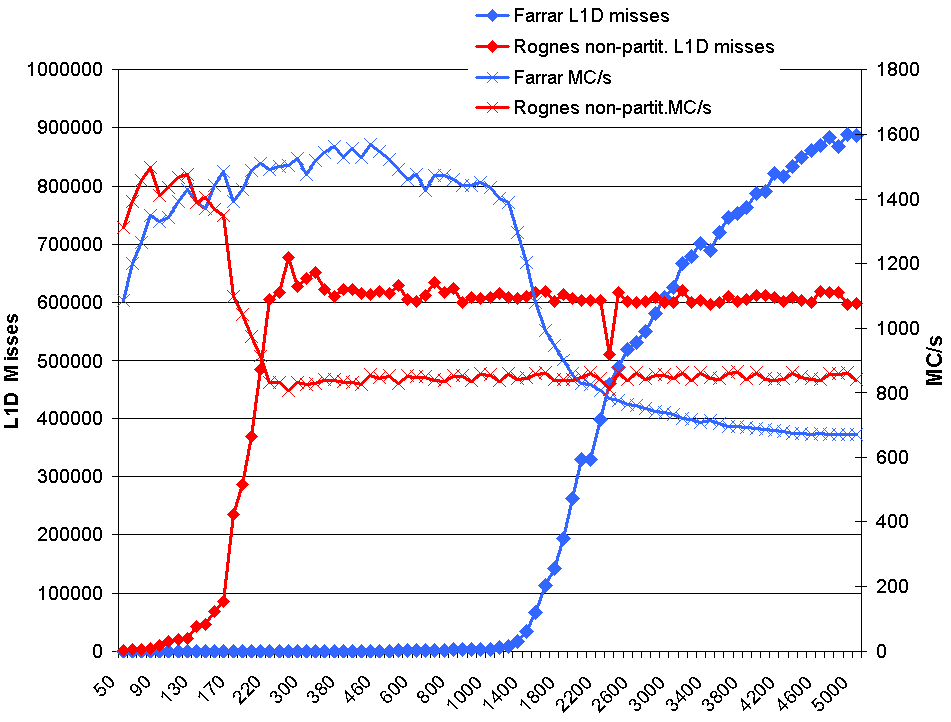
\includegraphics[width=16cm]{graphics/cache-misses-nonpart.png} 
	\caption[Cache profiling of non-partitioned models]  {Results of cache profiling of HMMER's Farrar-based ViterbiFilter, and the Rognes-based COPS, with a 32KB L1D cache. Measured in millions of cells computed per second (MC/s) and L1 data cache misses.}
	\label{cache-misses-nonpart}
\end{figure}

The theoretical estimates point to \emph{critical point} of full L1D utilization around $\sim$1470 for ViterbiFilter and $\sim$167 for COPS, for 32KB L1 data caches. These points coincide rather well with the observed spikes in cache misses and drops in performance, which figure strongly correlated in the results:

\begin{itemize}[noitemsep,nolistsep]

\item Rognes-based COPS: from a M of 120 to 220, there is a 26000\% increase in cache misses, and a 44\% drop in performance. Both the performance and the number of misses stabilize for M $>$ 220.

\item Farrar-based ViterbiFilter: between a M of 1200 and 2300, the number of misses rises 50000\% with the performance falling 43\%. Both the performance and the cache misses continue to deteriorate for longer models, although at a slower pace.

\end{itemize}

So, for practical applications, where the model length rarely exceeds 2000, COPS had a considerable memory handicap, which left it sorely uncompetitive vis-a-vis the striped ViterbiFilter. The graphic shows how the striped version was 70\% faster than the inter-sequence version for Ms between $\sim$180 and $\sim$1400. For models exceedingly long, starting with Ms $>$ 2400, COPS is again competitive and was able to achieve a small speedup against the HMMER implementation.





\subsection{Partitioning the Model}

In order to solve the cache efficiency problem, it was devised a \emph{loop-tiling} strategy based on a partitioning of the model states, that sought to limit the amount of memory required by the core loop. The normal model states are split in blocks of maximum \emph{M.P.} states, and the blocks are iterated over in a new outermost-loop. This corresponds to a standard \emph{loop-tiling} (a.k.a., \emph{strip-mining}) strategy, illustrated by the pseudo-code in \autoref{table-partitioning-comp}.

\begin{table}[htb!]
\centering
\caption[Inner loop code, before and after partitioning] {Comparison of the inner loop code, before and after partitioning the Model}
\label{table-partitioning-comp}

\begin{tabularx}{\textwidth}{ |X|X| }
\hline
Original code, non-partitioned  &  Strip-mined code, partitioned   \\ \hline

\begin{algorithmic}
\LeftComment Loop through the sequence symbols
\For {$i \gets 1 \textrm{ to } SequenceLength \ (L) $} 
	\State ...		

	\LeftComment Loop through the model state-triplets
	\For {$i \gets 0 \textrm{ to } M-1 $} 
		\LeftComment Core Viterbi code
		\State ...
	\EndFor
	
	\LeftComment Update the special states
	\State ...	
\EndFor
\end{algorithmic}

&
\begin{algorithmic}
\LeftComment  Loop through the partitions
\For {$i \gets 1 \textrm{ to } Npartitions $} 
	
	\LeftComment Loop through the sequence symbols
	\For {$i \gets 1 \textrm{ to } SequenceLength \ (L) $} 
	
		\State Load\_Data\_From\_Last\_Partition(i)
		\State ...		

		\LeftComment Loop through the state-triplets
		\LeftComment of the current partition

		\For {$i \gets 0 \textrm{ to } MP $} 
			\LeftComment Core Viterbi code
			\State ...
		\EndFor
	
		\LeftComment Update the special states
		\State ...	
		\State Store\_Data\_For\_Next\_Partition(i)
	\EndFor
	
\EndFor
\end{algorithmic}

\\ \hline
\end{tabularx}
\end{table}



The outer loop (new middle loop) over the sequences mostly re-uses the same memory locations (except for emission scores), which are accessed in the inner core loop, so these locations should be kept in close cache.
By limiting the model states loop to a maximum of \emph{MP} state-triplets, we can effectively guarantee that the whole sequence loop (the middle loop in the new layout) does not access more than roughly $\sim$ $(176 \times M + 320)$ bytes (disregarding the emission scores). The memory required by the inner loop is then cached in close memory, and repeatedly accessed over all the sequence loop while in cache, thereby reducing drastically the occurrence of cache misses.
The maximum partition length, \emph{MP}, is adjusted to achieve an optimal cache occupation, one that fills the available capacity of the closest data cache up to its limit.

There are two memory blocks which cannot be \emph{strip-mined} and thus degrade the performance of this optimization:

\begin {itemize}

\item Emission scores, which must be refreshed (re-computed) for each new round of sequence tokens. These values are only accessed once, so it is counter-productive to consider their cacheability.

\label{prefetching}
An attempt was made to prevent their loading into cache, by using the Intel \emph{software prefetch} instructions for non-temporal access, which tell the processor that the data is \emph{non-temporal} (i.e.; will never be reused) and thus should not evict other data from the cache. 
However, the non-temporal prefetches could not improve on the hardware prefetching already done by the processor, since the data access patterns are very regular (continuous actually). The number of LLC caches misses (i.e. for the larger L2 and L3 caches) is practically null.
% helper threads e prefetching n tem impacto

%An attempt to further exploit the parallelization potential of modern processors using Hyper-threading also proved infertile, actually yielding slightly slower code for Intel processors. In the case of AMD processors, the improvement from hyper-threading was very small. This shows how little time the program spends stalled, waiting for resources. 

\item Dependencies that must be exchanged between partitions. The last Match, Insert, and Delete contributions from each partition have to be carried on to the next partition, and so they have to be saved at the end of each partition. Each partition receives as input one line of previous states, with one state-triplet for each 8-fold round of sequences, and produces as output another line of values to the next partition. 

These dependencies can be minimized to 3 values per sequence round (vE, Mnext, and Dcv) after re-factoring the core code and moving the computation of Mnext with the 3 state dependencies to the end (\autoref{table-refactor-comp}).

\begin{table}[htb!]
\centering
\caption[Inner loop code, before and after refactoring the Match dependencies] {Comparison of the inner loop, before and after refactoring the Match computation to minimize the number of dependencies}
\label{table-refactor-comp}

\begin{tabularx}{\textwidth}{ |X|X| }
\hline

Original code	&  Refactored code \\ \hline

\begin{algorithmic}
	\LeftComment Loop through the model state-triplets
	\For {$i \gets 0 \textrm{ to } M-1 $} 

		\State $ Mnext \gets Max
					\begin{cases}
						vB + t_{BM}(k)	\\
						Mpv + t_{MM}(k)	\\
						Ipv  + t_{IM}(k)	\\
						Dpv + t_{DM}(k)	\\
					\end{cases} $ \\
		\State $ Mnext \gets Max(Mnext, e_{match}(k)) $

		\State $ vE \gets Max(vE, Mnext) $		
		\State $ Dpv \gets Dmx(k) $
		\State $ Ipv  \gets Imx(k)  $
		\State $ Mpv \gets Mmx(k) $
		\State $ Mmx(k) \gets Mnext $
		\State $ Dmx(k) \gets Dcv   $
		
		\State $ Imx(k) \gets Max
					\begin{cases}
						Mpv+  t_{MI}(k+1)	\\
						Ipv +  t_{II}(k+1)	\\
					\end{cases} $ \\

		\State $ Dcv \gets Max
					\begin{cases}
						Mnext +  t_{MD}(k+1)	\\
						Dcv +  t_{DD}(k+1)	\\
					\end{cases} $ 
	\EndFor
\end{algorithmic}
&
\begin{algorithmic}
	\LeftComment Loop through the model state-triplets
	\For {$i \gets 0 \textrm{ to } M-1 $} 

		\LeftComment Use partial value of Mnext
		\State $ Mnext \gets Max
					\begin{cases}
						Mnext \\						
						vB + t_{BM}(k)	\\
					\end{cases} $ \\
		\State $ Mnext \gets  Max(Mnext, e_{match}(k)) $

		\State $ vE \gets Max(vE, Mnext) $		
		\State $ Dpv \gets Dmx(k) $
		\State $ Ipv  \gets Imx(k)  $
		\State $ Mpv \gets Mmx(k) $
		\State $ Mmx(k) \gets Mnext $
		\State $ Dmx(k) \gets Dcv   $
		
		\State $ Imx(k) \gets Max
					\begin{cases}
						Mpv+  t_{MI}(k+1)	\\
						Ipv +  t_{II}(k+1)	\\
					\end{cases} $ \\
		\State $ Dcv \gets Max
					\begin{cases}
						Mnext +  t_{MD}(k+1)	\\
						Dcv +  t_{DD}(k+1)	\\
					\end{cases} $ 

		\LeftComment Partial computation of Mnext
		\State $ Mnext \gets  Max
					\begin{cases}
						Mpv + t_{MM}(k)	\\
						Ipv  + t_{IM}(k)	\\
						Dpv + t_{DM}(k)	\\
					\end{cases} $ \\
	\EndFor
\end{algorithmic}
\\ \hline
\end{tabularx}
\end{table}

\end {itemize}


\begin{figure}[htb!]
	\centering
	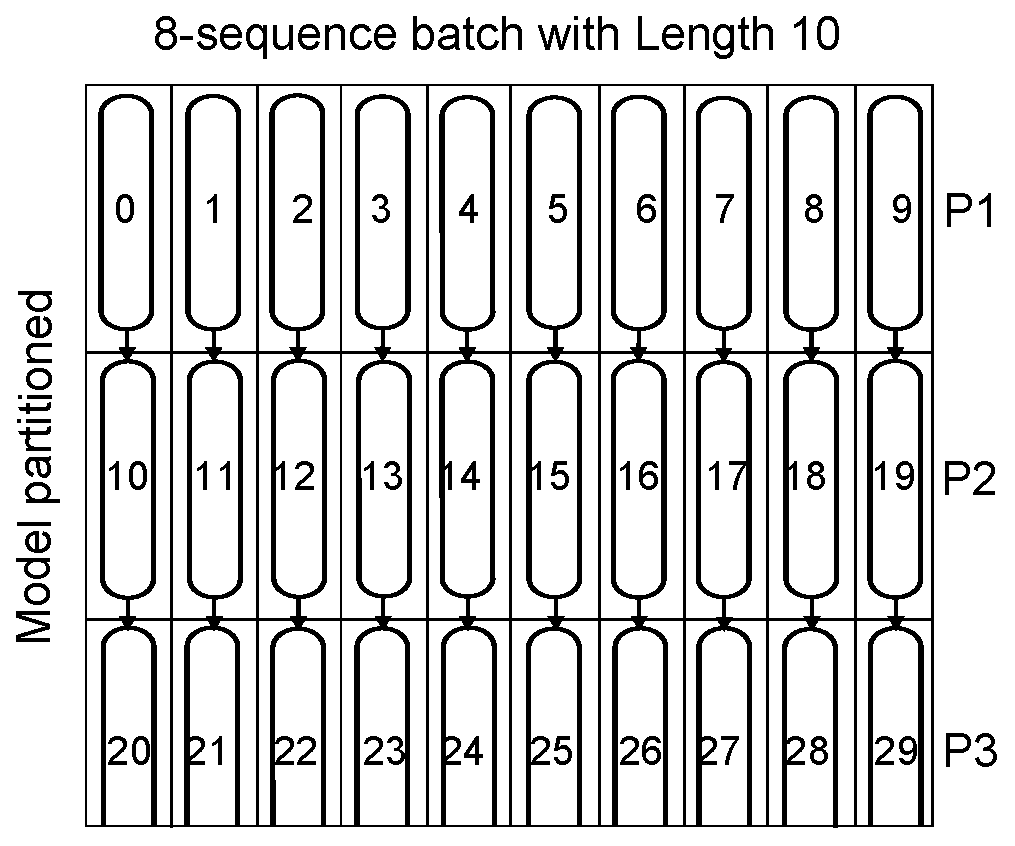
\includegraphics[scale=0.56]{img/partitions.eps} 
	\caption[Processing order in a partitioned model] {Processing pattern of the adopted partitioned model,with an 8-sequence batch of length 10. The numbers represent the processing order of each partition. The arrows show the inter-partition dependencies.}
	\label{figure-partitions}
\end{figure}

The processing order of the partitions is shown in \autoref{figure-partitions}.



\subsection{Problems of Model Partitioning}

There are some restrictions to the applicability of model partitioning however. The computation of each symbol-tuple through the model must be independent between each other. In particular, it must not depend on the final result of the previous symbol-tuple, which is the case for multihit alignments (alignment of the model multiple times against a sequence target). Therefore, the model can only be partitioned for unihit alignments (HMMER's 'uni-local mode'). In unihit alignments, the J special state, which encodes the token-to-token dependencies, is disabled.

The partitions used must necessarily have a length multiple of 8, to accommodate the loop step of 8 unrolled states. As a result, the model must be expanding up to a length also multiple of 8, by padding with dummy states and scores. The dummy scores are all set to -infinity so that they do not affect the result. The extra states add a slight performance penalty of extra computation.



\subsection{Determining the Optimal Empirical Partition Length}

Overall, the partitioned COPS implementation has an expected memory footprint of around $240*M + 900$ bytes (corresponding to the original memory requirements of the non-partitioned COPS, plus the additional arrays that are required to store the inter-partition dependencies). It can thereby be estimated the value for the maximum partition length ($MP$) as the maximum model length that limits the memory footprint to the size of the L1D. Hence the value of $MP$ can be determined by following the formula: $ MP = \frac{\displaystyle L1Dsize - 900}{\displaystyle 240} $.

Apart from a slight skew towards smaller lengths, justified by the sharing of the L1D cache with other variables not correlated with this processing loop, these estimated $MP$ values coincide very consistently with the best partition lengths that were experimentically observed:
\begin{itemize}[noitemsep,nolistsep]
\item 112 to 120 states, for 32KB L1D CPUs, (e.g. Intel Core, Core2, Nehalem, Sandy Bridge, Ivy Bridge and Haswell);
\item around 48  states, for 16KB L1D CPUs, (e.g. AMD's Opteron Bulldozer and Piledriver);
\item 216 to 224 states, for 64KB L1D CPUs, (e.g. AMD's Opteron K8, K10, Phenom I and II).
\end{itemize}

%These experimental values confirm the theoretical estimates of the L1D cache size limits, and its impact on inner loop data (see \autoref{table-memory-comp}).
%It was also observed that the size and policies of the outermost cache levels (usually L2 and L3 shared between cores) also affect the performance....
%Other processors will naturally have a different optimal value, mainly depending on the cache architecture (levels, policies and sizes of caches).



\subsection{Evaluation after Partitioning}

After partitioning, the overall performance behaved remarkably as expected, maintaining the same level of caches misses and computation speed for any model length:

\begin{figure}[h!]
	\centering
	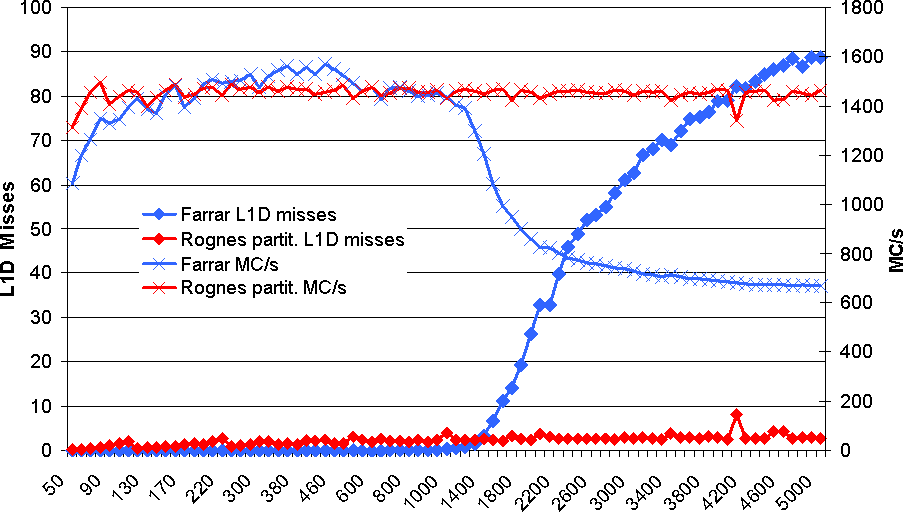
\includegraphics[width=16cm]{graphics/cache-misses-part.png} 
	\caption[Partitioning performance results] {Results of cache profiling of HMMER's Farrar-based ViterbiFilter, and the new partitioned COPS. Measured in millions of cells computed per second (MC/s) and L1 data cache misses.}
	\label{cache-misses-part}
\end{figure}

As a result, COPS managed to be slightly faster than HMMER's ViterbiFilter for models up to $\sim$1200, after which the COPS program quickly gains a close to 2-fold speedup over ViterbiFilter, due to the latter's cache degradation.

Compared to the non-partitioned COPS code, the partitioned version was about 42\% faster for long models ($\sim$1000) \emph{before refactoring the inner loop code}. After refactoring the auxiliary storage arrays (Mpv, Ipv, Dpv), the improvement was of 49\%. The complete pseudo-code of this final version is presented in \cref{code-complete} and \cref{code-compute}.




\section{Batches of Sequences with varying lengths}

Since the program runs with 8 parallel sequences in lock-step, there is a problem when the sequences have different lengths. The program must then either ignore the shorter sequences and continue until all sequences are completed (the static approach), or feed in new sequences to replace the finished ones, while the algorithm is running (the dynamic approach used by Rognes). 

The two possible approaches were implemented in this work, and their performance compared:

\begin{itemize}

\item \textbf{ Static approach: restarting the execution every time to load new sequences }
%\paragraph{Static approach: restarting the execution every time to load new sequences}

The sequences are padded with dummy valid symbols (e.g.; any residue) up to the length of the longest sequences, for each new group of sequences processed. The dummy residue maps to a score array of $-\infty$ scores. These emission scores cancel the updates of vE by the Match states $M$ when they are added to the computation of $M$.

In the 32-bit floating point implementation, additional concerns are required: the C $\rightarrow$ C transition cannot be eliminated with dummy scores. It was necessary to mark where each sequence terminates (i.e. its length), compare the limit length in each iteration, and then, by numeric manipulation, nullify the C $\rightarrow$ C transition for iterations beyond the limit length.

The wasted computation incurred by the dummy symbols was evaluated with a practical-use database (NRDB90) and found to be minimal: it accounted for less than 0.01\% of the total computing effort.
% Besides this penalty of redundant computation, there are additional drawbacks to this approach. Estao no texto abaixo do itemize


\item \textbf{ Dynamic approach: runtime swapping of sequences }
% \paragraph{Dynamic approach: runtime swapping of sequences}

The Dynamic swapping method was chosen by Rognes for his Swipe tool. In this approach, the sequences are checked in each iteration of the outer loop (loop over sequence symbols) to determine if any has reached its end. Those that have, are exchanged with the next database sequence, and the appropriate SSE vector elements in the auxiliary data arrays are reset to $-\infty$.

\end{itemize}


The performance of both methods was evaluated with both a randomized dataset of multiple-length sequences, and the NRDB90, whose sequences have more disparate lengths. On both tests, the Static approach proved to be about $\sim$60\% faster than the dynamic approach.

Furthermore, the Rognes dynamic method has a few limitations, which inhibits its use in the present work:

\begin{itemize}[noitemsep,nolistsep]
\item The sequence loop must be the outer-most loop, and by consequence it would not be possible to employ the Model partitioning optimization.
\item The parametrization of the model targeted to each particular sequence Length would equally prove impossible to conduct, since the entire database must be evaluated in a single execution run, without the possibility of re-starts and re-parameterizations.
\end{itemize}

Even if the swapping method were more efficient, these two limitations are enough to seal the decision of instead using the re-starting method in COPS.

However, with the static re-starting method, there is also an additional source of non-negligible scoring errors in the mis-parametrization of the sequences in the group. Before each execution of the algorithm, the model is reconfigured with the average sequence Length value among the 8 sequences. In particular, the re-configuration computes the transition scores of the special states. Since 8 sequences are processed in lock-step, if their lengths differ, the shorter sequences will yield slightly biased scores. This error can be minimized by first sorting the database sequences, which for practical large databases results in an uniform length for most 8-sequence batches. The re-configuration of the model is a very short step, and does not cause any measurable performance penalty.

The sorting step was done by the standard C implementation of the Quicksort algorithm. Its runtime cost was measured, and determined to be negligble in the context of the application. It took less than 0.01\% of the overall runtime, even when sorting large databases with either many small sequences, or fewer but larger sequences.





\section{Multi-threading the partitions}
\label{Multi-threading the partitions}

After having a partitioned model, each partition can be seen as a 'chunk' of data to process. This data layout seems particularly suitable for an additional level of paralellization: multi-threading using a wave-front model of partitioned chunks. From the start, the parallel speedup over the number of threads would expectedly never reach linear growth (mainly due to the unavoidable synchronization and communication between threads). Still, this second parallelization level is an interesting improvement, which could be applied to other areas (e.g.; single tasks that cannot be linearly decomposed into independent threads).


With a partitioned model, it is possible to add \ac{SMP} multi-threading to parallelize the partitioned chunks. Some number, $N$, of partitions are simultaneously processed by $N$ threads, following a wave-front pattern: each thread starts its assigned partition of the $i$-th sequence residue when the previous thread has finished the previous partition of the same $i$-th sequence residue (\autoref{wave-front-model}). The computing pattern is thus 1) left-to-right (ascending by sequence index), and 2) top-to-down (ascending by model state index).

\begin{wrapfigure}{r}{0.3\linewidth}
%    \resizebox*{0.3\columnwidth}{!}{ \includegraphics{img-hmm/wave-front-model.eps} }
	\includegraphics[width=1.0\linewidth]{img-par/wave-front-model.eps}
	\caption[Multi-threaded Wave-front pattern] {Multi-threaded Wave-front pattern. Blocks are processed concurrently in a diagonal pattern (same color for concurrent partitions). }
	\label{wave-front-model}
\end{wrapfigure}

The main-master thread has some special tasks that distinguish it from the worker-slave threads: it is the only thread responsible for loading the sequences, resetting the control and synchronization flags, and re-configuring the model.

There are two synchronization concerns involved in the multi-threaded wave-front strategy: synchronization of all threads at the start of the algorithm (since it is run multiple times using the same $N$ threads), and synchronization of data between threads processing inter-dependent chunks. These two concerns will be explained in detail in the following subsections.


\subsection{Execution call synchronization}

The first level of synchronization concerns the sequentiality of calls to the algorithm, each call running with the same threadpool, requiring synchronization of all threads before starting each new execution of the algorithm. The synchronization here is essential to allow time for the main thread to do its preparation work between runs. On the other hand, it is desirable that the synchronization be as efficient and lightweight as possible.

A few methods were tried, which either did not ensure the proper synchronization, or were not optimally efficient:

\begin{itemize}

%\item Mutexs and signals
%
%\begin{algorithm}[htb!]
%\caption{ - Pseudo-code of synchronization method with mutexes and signals}
%\label{code-mutexs}
%
%\begin{algorithmic}
%\State MutexLock(synchMutex)
%\If{MASTER}
%	\State ConditionBroadcast(synchCond)
%\Else 
%	\State ConditionWait(synchCond, synchMutex)
%\EndIf
%\State MutexUnlock(synchMutex)
%\end{algorithmic}
%\end{algorithm}
%
%This method fails because it requires the main thread to be the last entering the mutex, which usually happens, but it's not guaranteed.


\item Synchronization barrier from Pthreads library

This approach consists of the primitive pthread\_barrier from the POSIX Pthread library, which acts on a 'barrier' variable initialized with the desired number of threads. When the method 'Wait' is called by a thread, it is blocked by in the barrier until all threads have called the same method. 
This primitive achieves the synchronization requirement of this project, but it is slower than other methods.


\item Per-thread semaphores

\begin{algorithm}[htb!]
\caption{Pseudo-code of synchronization method with Semaphores}
\label{code-semaphores}

\begin{algorithmic}
	\LeftComment Declaration:
	\State Semaphore synchSems[NTHREADS]
		
	\LeftComment Initialization:
	\For{$i \gets 0 \textrm{ to } Nthreads $} 
		\State SemaphoreInit(synchSems[i], 0)
	\EndFor
	
	\LeftComment Worker:
	\State SemaphoreWait(synchSemaphores[myThreadId])
	
	\LeftComment Main:
	\For{$i \gets 0 \textrm{ to } Nthreads $} 
		\State SemaphorePost(synchSemaphores[i])
	\EndFor
\end{algorithmic}
\end{algorithm}


The semaphores are initialized with a value o 0. To start each run, the main thread signals each worker thread that it can start, using the \emph{Post} method. Each worker thread calls the \emph{Wait} method on its corresponding semaphore. This method will either block and wait if the main thread hadn't signaled it yet, or consume one value and proceed if otherwise. The workers that are waiting on the semaphores are woken up by the main thread signals.

The semaphores technique works but it is again slower than other methods.



\item Per-thread start flags

This method uses an array of simple synchronization flags (integers), one per thread, wherein each thread may wait for a command from the main thread.

\begin{algorithm}[htb!]
\caption{Pseudo-code of synchronization method with Per-thread start flags}
\label{code-startflags}

\begin{algorithmic}
	\LeftComment Worker:
	\While { syncFlags[myThreadId] is False }
		\State YieldCPU()
	\EndWhile
	\LeftComment after leaving the loop, and seeing a True flag, reset it to False:
	\State syncFlags[myThreadId] = False

	\LeftComment Main:
	\For{$i \gets 0 \textrm{ to } Nthreads $} 
		\State syncFlags[i] = True
	\EndFor
\end{algorithmic}
\end{algorithm}

Again, this is a functional and lightweight method, but it was deferred in exchange for a more slightly better approach.

\end{itemize}

In the end, the chosen method was a variation of the Per-thread start flags, that uses a single global execution counter and per-thread local counters:

\begin{algorithm}[htb!]
\caption{Pseudo-code of synchronization method with Per-thread local counters}
\label{code-counters}

\begin{algorithmic}
	\LeftComment Main:
	\State Inc globalExecCounter

	\LeftComment Worker:
	\State myExecCounter = 0
	\While { True }
		\State Inc myExecCounter
		\While { globalExecCounter $\neq$  myExecCounter }
			\State	YieldCPU()
		\EndWhile
		\State Call DoWork()
	\EndWhile

\end{algorithmic}
\end{algorithm}


The worker waits (yielding the CPU) until its local replica counter matches the value of the global counter, whose value is only set by the main thread.
There are no data consistency concerns here, simply because outdated values of the global counter will not cause undesired behavior, such as workers' early starts. The only problematic effect of out-of-date values is possibly additional wait cycles for the workers.

Two simple benchmarks were used to evaluate the relative performance of each synchronization method: a first benchmark (\autoref{synch-computation}) consisting of a small model and small generated random sequences ($\sim$100 residues each); and a second benchmark (\autoref{synch-nocomputation}) that stressed the synchronization primitives alone, with no computation whatsoever.

\begin{figure}[htb!]
    \begin{minipage}{0.48\linewidth}
		\centering
		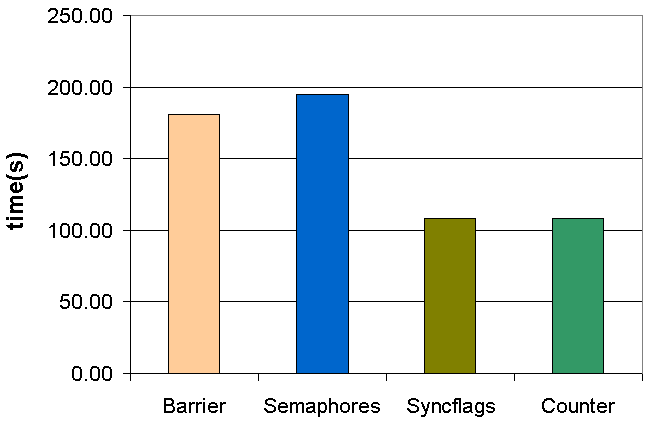
\includegraphics[width=7.5cm]{graphics/synch-computation.png} 
		\caption[Synchronization Evaluation with computation] {First benchmark: COPS code with a 100-length model, 4 threads, and 800K 100-length sequences.}
		\label{synch-computation}
    \end{minipage}
    \hspace{0.04\linewidth}
    \begin{minipage}{0.48\linewidth}
		\centering
		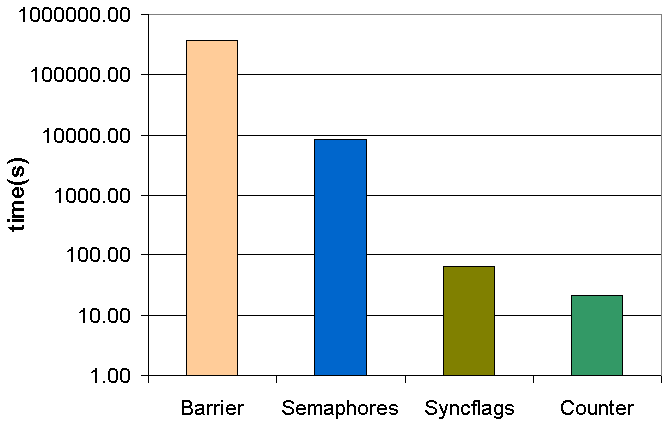
\includegraphics[width=7.5cm]{graphics/synch-nocomputation.png} 
		\caption[Synchronization Evaluation without computation] {Second benchmark: only synchronization primitives, in $80K \times 80K$ rounds. Logarithmic scale.}
		\label{synch-nocomputation}
    \end{minipage}
%	\caption{Relative performance of the various synchronization methods. Tested on a quadcore Intel Core2duo.}
\end{figure}


These results show that the Counter method is indeed the most efficient solution. Note the logarithmic scale on the second benchmark, clearly illustrating the disproportionate efficiency of the no-locks methods vis-a-vis the locking approaches.

Finally, it was evaluated the overall percentage of idle thread time incurred by the chosen method (global Counter + local counters). A battery of tests was run, starting from sequences with a large amount of wasted computation lines due to partitioning, and down to sequences with no wasted computation. The determined result was that the total idle thread, cumulative of the 4 threads used, ranged from < 1\% to a maximum of 5\% in the worst case, with an average between 0\% and 2\%. These values are reasonable and quite positive for the average case.


	
\subsection{Partition synchronization}

The second level of synchronization concerns the exchange of data between threads processing adjacent partitions. Namely, each thread must send data to the thread processing the succeeding partition, independently for each sequence index. Moreover, each thread must block itself while it is waiting for data from the preceding partition, and this procedure repeats for each and every sequence index. The synchronization overhead is reduced by the decomposition by sequences indices, resulting in relatively small work-chunks of size $PartitionLength \times 1$.

To implement this synchronization requirement, it was chosen a simple and efficient solution: 
\begin{itemize}
\item $Nthreads$ arrays of flags, one for every pair (partition, sequence symbol), wherein threads can wait and signal one another. The wait is implemented by yielding the CPU and the signaling is done by setting the flag.

\item Unique arrays (with length equal to the sequence length) for the data that needs to be exchanged.
Only one array is needed for each type of data, because only one transfer of data can occur at any given time for each sequence symbol (i.e.; the data is propagated only one thread at a time, every time the active thread finishes and passes its data to the next partition thread). Only one thread is active processing a sequence index at a given time, any other thread is either in a previous index or waiting on the preceding partition thread.
\end{itemize}

The chosen synchronization technique has the precious benefit of not using any locks or blocking primitives.
No memory barriers are needed, because stale data is not a problem for the program. Data that is not updated will cause no consistency problems, rather it will merely lead to more waiting (yielding) cycles. The flags are only reset by the master thread, before starting the algorithm.

%Volatiles parece que tambem nao sao precisos. Mas nao tem impacto na performance.
	

\subsection{Computing the Practical Threaded Partition Length}

A relevant issue to consider is what partition length should be used in each case? This practical partition length differs from the theoretical optimal length by taking into account the computation effort that is wasted by idle threads when the partitions are not evenly divisible by the threads.

The optimal length depends on a few variables: model size, number of threads, and optimal partition length (which is used as a maximum threshold for the practical length), with the stated goal of finding a partition length that maximizes the effective thread use.

\begin{enumerate}

\item It is computed the number of minimum (i.e. assuming the threshold length) total chunks required to cover the complete model, and that are a multiple of the number of threads:
	$MinNchunks = roundtop(\frac{M}{MaxPartLength}, Nthreads)$

\item This minimum number of chunks is used to compute the practical partition length (which has to be a multiple of the SSE vector size, 8):
	$ PartitionLength = roundtop(\frac{M}{MinNchunks}, 8) $

\item The actual number of partitions is finally calculated based on the partition length chosen:
	$Npartitions = ceiling(\frac{M}{PartitionLength} ) $
	
\end{enumerate}

% AQUI podia-se falar do calculo do trabalho desperdicado

The partitions are then issued to the available threads, using static decomposition and a fixed pinning scheme that ensures the last partition belongs to the master thread (which has the last ThreadId). This is important because it is the master that deals with the algorithm terminations, and extracts and computes the final result.

The following formula was used to determine the start partition of each thread:
	$StartPartition = (Npartitions + myThreadId) \mod Nthreads $

	


%\cleardoublepage
\clearpage

		
